\documentclass[tikz]{standalone}
\usepackage{fontspec}
\renewcommand*{\familydefault}{\sfdefault}
\usepackage{standalone}
\usepackage{amssymb}
\usetikzlibrary{decorations}
%\usetikzlibrary{arrows.meta, decorations.pathmorphing, decorations.pathreplacing, shapes.geometric}
\usetikzlibrary{bayesnet}

\begin{document}
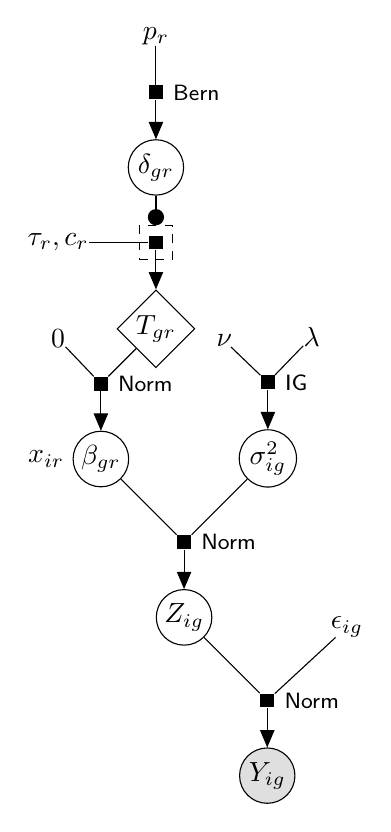
\begin{tikzpicture}%[font=\footnotesize, xscale=1.5]
    % 1st (bottom) level
    \node[obs] (Y) {\(Y_{ig}\)};
    \factor[above=0.5 of Y, label=right:Norm] {Y-factor} {} {} {};
    \node[latent, above left=1.0 of Y-factor] (Z) {\(Z_{ig}\)};
    \node[const, above right=1.0 of Y-factor] (epsilon) {\(\epsilon_{ig}\)};
    \factoredge {Z, epsilon} {Y-factor} {Y};

    % 2nd level
    \factor[above=0.5 of Z, label=right:Norm] {Z-factor} {} {} {};
    \node[latent, above left=1.0 of Z-factor] (beta) {\(\beta_{gr}\)};
    \node[const, left=0.1 of beta] (x) {\(x_{ir}\)};
    \node[latent, above right=1.0 of Z-factor] (sigma) {\(\sigma^2_{ig}\)};
    \factoredge {beta, sigma} {Z-factor} {Z};

    % 2nd level
    % beta
    \factor[above=0.5 of beta, label=right:Norm] {beta-factor} {} {} {};
    \node[const, above left=0.5 of beta-factor] (zero) {\(0\)};
    \node[det, above right=0.5 of beta-factor] (T) {\(T_{gr}\)};
    \factoredge {zero, T} {beta-factor} {beta};
    % sigma
    \factor[above=0.5 of sigma, label=right:IG] {sigma-factor} {} {} {};
    \node[const, above left=0.5 of sigma-factor] (nu) {\(\nu\)};
    \node[const, above right=0.5 of sigma-factor] (lambda) {\(\lambda\)};
    \factoredge {nu, lambda} {sigma-factor} {sigma};

    % 3rd level
    \factor[above=0.5 of T] {T-factor} {} {} {};
    \node[const] (tau-c) at (T-factor -| zero) {\(\tau_{r}, c_{r}\)};
    \factoredge {tau-c} {T-factor} {T};
    \node[latent, above=0.5 of T-factor] (delta) {\(\delta_{gr}\)};
    \gate {} {(T-factor)} {delta};
    \factor[above=0.5 of delta, label=right:Bern] {delta-factor} {} {} {};
    \node[const, above=0.5 of delta-factor] (p) {\(p_r\)};
    \factoredge {p} {delta-factor} {delta};

\end{tikzpicture}
\end{document}
